
\chapter{Fundamentação Teórica\label{chap:FundamentacaoMatematica}}

% Revisar a citação de motores elétricos CHAPMAN

% Resumo opcional. Comentar se não usar.
%\resumodocapitulo{Resumo opcional.}

\section{Revisão Bibliográfica}
\label{sec:revisaobib}

A idealização, construção e controle de braços robóticos montados sobre cadeiras de rodas é um foco de pesquisa amplo, 
sendo desenvolvidos projetos tanto na área comercial quanto na área de 
pesquisa universitária, resultando em diferentes produtos com focos distintos. 
É interessante estudar os tipos de tecnologias, características e funcionalidades
propostas nos diversos trabalhos desenvolvidos, tanto para tecnologias 
assistivas quanto para tecnologias semelhantes, para se ter uma boa base
no desenvolvimento de um novo projeto, que busque apresentar algum 
diferencial frente às tecnologias já existentes.

Na Universidade de Brasília, já foram desenvolvidos projetos envolvendo a adaptação, controle e instrumentação de cadeiras de rodas para deficientes. 
Uma vez que os braços robóticos são montados sobre estas, é importante analisar estes projetos a fim de estudar tecnologias de alimentação e acoplação para o braço 
proposto. Foi apresentado, em conjunto com a Universidade Federal de Pernambuco e outras partes, um \textit{kit} de automação para cadeiras de rodas convencionais 
\cite{vidal2010desenvolvimento}, sendo este de extrema importância por já demonstrar as dimensões e limitações básicas de uma cadeira de rodas convencional, 
o tipo e posicionamento do circuito de alimentação e componentes eletro-eletrônicos comumente empregados neste tipo de projeto.
O trabalho apresentado em \cite{francisco2019interface} foca no desenvolvimento de uma interface para que o operador possa controlar a cadeira de rodas
de forma satisfatória, fornecendo ideias para uma interface viável também para o controle do braço robótico a ser acoplado neste tipo de cadeira de rodas.

Os projetos citados demonstram que é comum a utilização de baterias 
automotivas como fonte de energia ao sistema de locomação, podendo esta mesma bateria
servir também como alimentação para um braço robótico acoplado à cadeira 
de rodas, fornecendo uma tensão nominal comum de 12V.
Também é notável a escolha por motores de corrente contínua, ou simplesmente
motores DC, para este tipo de tecnologia, com acionamento controlado através de 
circuitos do tipo ``Ponte H''.

Embora não tenham sido encontrados especificamente projetos acerca de WMRA na Universidade de Brasília, foram identificados projetos de braços robóticos
construídos para outros fins, sendo uma análise desses imprescindível para se ter conhecimento acerca do tipo de atuadores e sensores comumente empregados em 
braços robóticos no geral.

%\subsection{Manipulador robótico didático}
Um manipulador didático, desenvolvido em \cite{wattylas2015didatico} e aprimorado em \cite{marconi2016didatico}, apresenta uma estrutura semelhante a do trabalho base
deste projeto, em relação ao posicionamento relativo das juntas iniciais, como pode ser visto na figura \ref{fig:manipulador-didatico}.

\begin{figure}[ht]
\caption{Modelagem do robô didático \cite{wattylas2015didatico}.}    
\begin{centering}
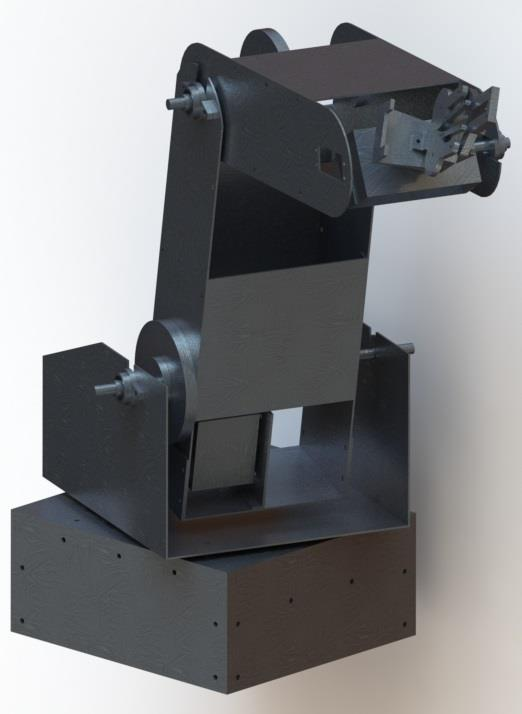
\includegraphics[width=0.5\columnwidth]{images/fundamentos/manipulador-didatico.png}
\par\end{centering}

\label{fig:manipulador-didatico}
\end{figure}

O projeto em questão tem como foco a interação entre o braço e pessoas com a finalidade de estimular e auxiliar o aprendizado no ramo da engenharia.
Embora este manipulador não seja do tipo WMRA, os circuitos de 
acionamento projetados e o método de controle desenvolvido podem ser 
levados em consideração no projeto atual, demonstrando a importância da
análise deste sistema.
A estrutura do robô apresenta uma base e três juntas com eixos paralelos
em sequência, em convergência com o modelo base para este projeto, desse modo,
pontos de desenvolvimento acerca da cinemática inversa podem ser comparados
e reutilizados.

Neste trabalho são expostas também a escolha por motores de passo em 
algumas juntas e uma ideia de \textit{driver} para controle destes, 
levantando a possibilidade de uso desse tipo de motores em projetos 
de manipuladores robóticos.

%\subsection{WMRA - USF}
Foi desenvolvido na \textit{Universisty of South Florida} um robô com motivações semelhantes à deste projeto \cite{kevin2005WMRA}, buscando atender às 
necessidade de pessoas com mobilidade reduzida e redução de custos deste tipo de tecnologia. O manipulador final apresenta 7 graus de liberdade, onde todas as
juntas são acionadas por motores DC escovados servo-controlados e controladas em conjunto através de placas 
controladoras baseadas na arquitetura PIC.
Uma foto do braço construído pode ser vista na figura \ref{fig:wmra-usf}.

\begin{figure}[ht]
\caption{Braço robótico completo construído na USF \cite{kevin2005WMRA}.}    
\begin{centering}
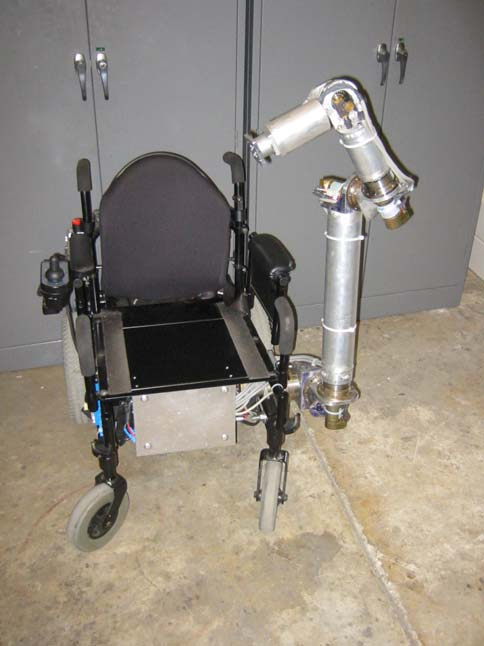
\includegraphics[width=0.5\columnwidth]{images/fundamentos/wmra-usf.png}
\par\end{centering}

\label{fig:wmra-usf}
\end{figure}

O manipulador final, com uma massa de 12.5kg, tem a capacidade de atingir uma altura máxima de 1.37m acima do chão e suporta uma carga, ou \textit{payload}, de até
6kg. Há dois pontos principais que devem ser observados no resultado final obtido pelo 
projeto citado, no que diz respeito a este projeto. 
O primeiro ponto de interesse está na utilização de caixas de engrenagens
harmônicas, que permitem uma alta relação de transmissão de torque, facilitando
a escolha dos motores utilizados.
O segundo ponto está nas unidades de controle aplicadas, apresentando 
características importantes no controle de motores DC, como controle PID
de posição e velocidade, comunicação RS-485 e leitura integrada de diversos
sensores, fatores que também devem ser levados em consideração no desenvolvimento
deste projeto.

Além dos modelos de braço robótico resultantes de estudos em universidades, 
há diversos tipos de modelos de WMRA existentes no mercado, apresentando 
geometrias, método de atuação, alcances e \textit{payloads} diferentes. 
O estudo desses modelos fornece uma boa base para novos projetos, podendo 
o modelo proposto ser comparado aos modelos comerciais a fim de se analisar 
a adequação da solução proposta ao mundo real.

Entre os modelos comerciais encontram-se o sistema JACO, construído pela empresa Kinova, o sistema MANUS e sua evolução iARM, desenvolvidos pela \textit{Assistive
Innovations} e o modelo \textit{Raptor}, fabricado pela \textit{Applied Resources} \cite{ktistakis2015survey}, onde cada um desses modelos pode ser levado em 
consideração na geração de especificações para um novo braço robótico com finalidade semelhante.
Em relação aos modelos comerciais, os fatores de comparação que mais
impactam este projeto seriam a velocidade linear atingível, tensão de 
alimentação, consumo e interface homem-máquina, outros fatores como alcance, peso e \textit{payload}
foram importantes no momento de decisão da estrutura mecânica no manipulador. 

Um estudo destes modelos demonstra que \textit{joysticks} são frequentemente 
utilizados como uma possibilidade de interface entre o operador e o robô \cite{capille2010kinematic},
sendo este modelo de interface adotado também na execução deste trabalho.

\section{Atuadores}
Em relação aos atuadores utilizados em manipuladores robóticos, há a possibilidade de emprego de atuadores do tipo hidráulico, pneumático e/ou eletromagnéticos, 
dentre outros, onde cada tipo de atuador apresenta pontos fortes e fracos para a aplicação em questão. 

Os atuadores hidráulicos são empregados geralmente por sua capacidade de gerar forças e torques elevados, com um controle simples, no entanto, embora os 
atuadores em si normalmente sejam compactos, é necessário uma grande quantidade de equipamentos extras para garantir o funcionamento e segurança destes, como
bomba, mangueiras, válvulas e acumuladores. Por sua vez, os atuadores pneumáticos apresentam uma capacidade de gerar forças um pouco inferiores àquelas atingidas 
por atuadores hidráulicos mas em velocidades mais elevadas, e também não necessitam de meios de contenção de líquidos, outrora utilizados em meios hidráulicos, 
porém, apresentam em geral um controle menos preciso com precisão afetada pela compressibilidade do ar e atrito interno dos atuadores \cite{hunter1991comparative}. 
Nestas duas classes de atuadores os mais utilizados são os atuadores lineares, porém há também os atuadores rotativos e atuadores do tipo músculo.

No que diz respeito aos atuadores elétricos, estes vem ganhando uma grande participação na aplicação em manipuladores, principalmente pela quantidade de 
alternativas de faixas de torque e velocidade, além de poderem apresentar um controle mais simples e fino. Entre os motores elétricos há aqueles operados
por corrente alternada e aqueles acionados por uma corrente contínua, sendo que a principal diferença entre estes encontra-se no método de controle
da velocidade de rotação. Os motores de corrente alternada, ou motores AC, são geralmente mais robustos e tem a sua velocidade controlada através da frequência
de oscilação da alimentação, sendo utilizados majoritariamente em aplicações com potência elevada e uma velocidade contínua com pequenas variações. Dentro da categoria de motores de corrente contínua existe uma diversa gama de modelos de atuadores, 
como motores DC de imã permanente, de excitação independente e em série, sendo diferenciados também pela presença de escovas ou não \cite{chapman2005electric}. 
Os motores DC podem apresentar um tamanho mais reduzido para aplicações mais simples, além de necessitarem de circuitos acionadores frequentemente mais simples em 
relação aos motores AC.

\section{Sensoriamento e Condicionamento}
Para se garantir eficiência e precisão durante a operação de um robô, é essencial a utilização de sensores, sendo neste ramo de pesquisa os sensores
divididos em sensoriamento interno, como no caso de medição da posicão, velocidade e torque das juntas, ou sensoriamento externo, como sensores próprios para 
visão, e medição de força e distância \cite{bajd2010robotics}.

Em um sistema de medição, geralmente são identificados quatro tipos de elementos, sendo os elementos do tipo sensor o primeiro desses. Usualmente são empregados
em conjunto com sensores elementos de condicionamento, processamento e de apresentação de dados, para garantir que a leitura desejada será devidademente medida
e tratada \cite{bentley2005principles}.

Na categoria de sensores que podem ser utilizados para se monitorar posicionamento as principais escolhas seriam os potênciometros, \textit{encoders} ópticos, 
sensores indutivos e de efeito \textit{hall}. Entre estes sensores de posicionamento, há aqueles que fornecem informações relativas à uma posição inicial e aqueles
capazes de fornecer uma informação acerca de um posicionamento absoluto mensurado \cite{bentley2005principles}. Sensores de toque, ou fim-de-curso, podem ser utilizados
a fim de se ter conhecimento do estado das juntas de um robô em determinada posição, auxiliando em um posicionamento correto no espaço.

Para se ter uma ideia do torque interno das juntas de um robô podem ser empregados também sensores do tipo \textit{hall}, no caso de juntas com motores elétricos, 
com o objetivo de se mensurar e auxiliar no controle da corrente que chega nos atuadores, diretamente relacionada com o torque resultante. A fim de mensurar ações de forças 
externas são comumente empregadas células de carga, que constituem um sistema de medição com extensômetros e condicionadores de sinal. O uso de extensômetros nos 
elos de um manipulador permite obter informações sobre ações externas e deformação que agem sobre estes, podendo estas serem usadas de modo a garantir uma maior
segurança durante a operação do manipulador.

Alguns fatores importantes na escolha de elementos sensores são a 
resolução, histerese, limiar de medição e zona morta dos mesmos, 
fatores estes que influenciam a acurácia e precisão da leitura. 
Instrumentos de medição do tipo \textit{encoder} e potenciômetros 
estão sujeitos a uma certa resolução, que é definida em \cite{doebelin2007measurement} 
como a menor quantidade possível de variação na entrada que resulta 
em uma mudança do valor de saída, sendo imprescindível escolher um 
dispositivo que forneça uma resolução boa o suficiente para que o 
posicionamento dos elos e juntas de um manipulador seja conhecido 
com baixa incerteza.

Demais instrumentos de tratamento de sinal também estão sujeitos a estas
condições de operação, conversores analógicos-digitais - ADC, por exemplo, possuem
uma resolução relacionada com a quantidade de \textit{bits} utilizados
na conversão de valores, sendo importante atentar-se a este tipo de 
elemento em um circuito de instrumentação \cite{bentley2005principles}. 
Esta relação de resolução pode ser vista na equação \ref{eq:res_adc}, 
onde a resolução foi indicada
por $\rho$ e $n$ indica a quantidade de bits disponíveis no conversor.

\begin{equation}
    \label{eq:res_adc}
    \rho = \frac{1}{2^n}
\end{equation}

Tratando-se de resolução, \textit{encoders} rotativos apresentam características
semelhantes aos conversores citados, por possuirem uma quantidade de posições  
que se equipara à quantidade de bits em um ADC. 
A resolução destes pode ser definida de acordo com
a equação \ref{eq:res_encoder}, onde $PPR$ identifica a quantidade de 
pulsos, ou posições, por revolução. Esta resolução pode ser aprimorada
incluindo-se uma relação de transmissão entre o eixo da junta e o sensor,
aumentando assim a escala de saída do sensor para uma mesma escala
de entrada, fazendo com que o mesmo valor na entrada possua uma gama maior
de relação com a saída, superando a resolução básica do sensor.

\begin{equation}
    \label{eq:res_encoder}
    \rho = \frac{2\pi}{PPR}
\end{equation}

Potenciômetros podem também estar sujeitos às limitações impostas 
pela resolução, como no caso de potenciômetros construídos com fios 
enrolados, no entanto, outros modelos, como os de plástico condutivo,
não estão sujeitos a estes efeitos \cite{bentley2005principles}.

Em relação à transmissão de sinais elétricos, o devido cuidado deve
ser tomado para evitar que ruídos e interferências afetem o sinal de 
modo a inserir erro no funcionamento geral do sistema. 
As fontes de ruído são divididas em internas e externas. Uma possível fonte de
ruído interna é a movimentação de cargas em elementos condutores 
devido à temperatura, por esse motivo este tipo de ruído é denominado 
ruído térmico, ou ruído de Johnson-Nyquist, sendo considerado uma forma de
ruído branco, por apresentar uma densidade espectral aproximadamente 
constante. Circuitos AC ou circuitos com chaveamento próximo ao sistema 
são, por sua vez, fontes comuns de ruído externo, 
podendo gerar transientes no sinal transmitido \cite{bentley2005principles}.

Os ruídos e demais interferências sobre um sistema elétrico podem ser 
considerados como em série, apresentando-se como uma fonte de 
diferencial de potencial entre o sistema emissor e receptor do sinal, 
ou de modo comum, onde os potenciais de ambos emissor e receptor estão
sujeitos a uma variação de potencial referente ao ruído que age sobre o sistema \cite{bentley2005principles}.

\begin{figure}[h]
    \caption{Interferência causada por múltiplos terras.}    
    
    \begin{centering}
        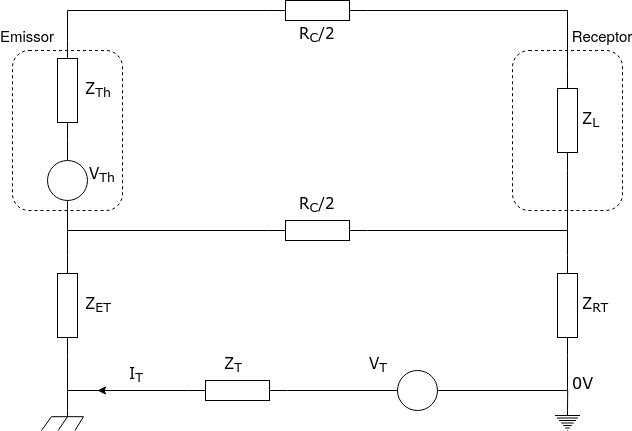
\includegraphics[width=0.7\columnwidth]{images/fundamentos/Interferencia.png}
    \par\end{centering}

    \label{fig:interferencia}
\end{figure}

A figura \ref{fig:interferencia} ilustra interferência causada pelo
problema comum de múltiplos terras, onde pontos que teoricamente deveriam
apresentar o mesmo potencial de 0V possuem entre si uma diferença de 
potencial, representada por $E_T$, causada por descarga de equipamentos ou quaisquer 
outros fatores. Esta diferença de potencial faz com que apareça no sistema 
uma corrente $I_T$, gerando tanto uma interferência de modo comum, ao 
induzir uma tensão sobre a impedância entre o receptor e o plano de terra
real, $Z_{RT}$ e um interferência em série, através da diferença de 
tensão que surge sobre a resistência do cabo $R_C/2$. Por esse motivo, é 
essencial que o sistema de medição seja conectado ao plano de terra em 
um único ponto, quando não é possível garantir o mesmo potencial no 
emissor e receptor \cite{bentley2005principles}.

Outro fator que pode afetar a integridade de sinais são as reflexões 
e distorções causadas por discontinuidades de impedância ao longo do 
caminho de transmissão. 
Quando um sinal elétrico encontra uma discordância entre pontos de 
diferentes impedâncias, parte dele será refletico de volta à origem,
causando ruídos de reflexão, resultando em uma degradação do sinal. 
A estratégia mais comum para evitar este tipo de reflexão consiste
na inserção de uma resistência próxima ao emissor do sinal, com o valor
necessário para que a soma das impedância dessa nova resistência com a
impedância interna do emissor sejam equivalentes à impedância da linha
de transmissão \cite{bogatin2010signal}. 

Dentre os métodos utilizados para redução dos efeitos de ruídos e 
interferências na transmissão de sinais, são notáveis a importância da
separação do circuito de medição de possíveis fontes de interferência,
como circuitos de potência, uso de técnicas de blindagem em cabos, como
transmissão por par de cabos trançados e/ou uso de camadas específicas de
blindagem, envio e recebimento de sinais diferenciais, isolamento entre
emissor e receptor e tratamento por meio de filtros \cite{bentley2005principles}.

Dentre os filtros implementados no tratamento de sinais encontra-se os
filtros passa-baixo, passa-alto, passa-banda e rejeita-banda \cite{irwin2010basic}. 
Os filtros passa-baixo são utilizados na atenuação de componentes de alta
frequência dos sinais, priorizando as variações de baixa frequência.
Este tipo de filtro é utilizado largamente quando há a necessidade de
filtrar sinais resultantes da mudança de estados de botões, removendo
em grande parte os efeitos de seus transientes mecânicos \cite{ganssle2004guide}.

\begin{figure}[h]
    \caption{Filtro RC.}    
    
    \begin{centering}
        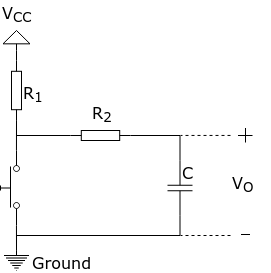
\includegraphics[width=0.3\columnwidth]{images/fundamentos/RCFilter.png}
    \par\end{centering}

    \label{fig:filtrorc}
\end{figure}

Normalmente assumindo o formato representado na figura \ref{fig:filtrorc},
um filtro RC garante uma variação mais bem definida para a saída do 
circuito através do descarregamento e carregamento do capacitor. 
A relação entre o valor de saída e valor de entrada depende do regime
onde se encontra o capacitor, carregamento ou descarregamento. 
As equações que regem esses regimes estão descritas nas fórmulas 
\ref{eq:filtrorc1}, para o carregamento, e \ref{eq:filtrorc2}, para o descarregamento.

\begin{equation}
    \label{eq:filtrorc1}
    V_O = V(t) = V_{CC}\left(1-e^{\frac{-t}{\tau}}\right)
\end{equation}

\begin{equation}
    \label{eq:filtrorc2}
    V_O = V(t) = V(t_0)\left(e^{\frac{-t}{\tau}}\right)
\end{equation}

Em ambos casos a constante de tempo $\tau$ é dada pela multiplicação 
entre a resistência equivalente do circuito e a capacitância, $\tau = RC$.
Nota-se que para o carregamento do capacitor a resistência total do
circuito equivale à soma das resistências de $R_1$ e $R_2$, já no 
descarregamento, somente $R_2$ influencia a constante de tempo. 

Amplificadores operacionais podem também ser usados no condicionamento
de sinais elétricos, sua impedância de entrada idealmente infinita 
evita pertubar o sinal nos terminais de entrada, por demandar pouca 
corrente.
A definição de um ganho em circuito pode também facilitar a leitura 
de sinais pequenos de tensão por equipamentos com baixa precisão, 
elevando um sinal na escala de millivolts para volts.

Quando da aplicação de um circuito integrado (CI) do tipo amplificador
operacional, alguns cuidados devem ser tomados em relação aos
comportamentos não ideais deste, ou imperfeições, 
como tensão e corrente de \textit{offset} \cite{sedra1998microelectronic}.
A rejeição de modo comum, ou CMRR, do inglês \textit{Common-Mode Rejection Ratio},
é uma característica que deve ser observada na aplicação deste tipo de 
CI, onde geralmente é desejado que seja amplificado unicamente a 
diferença de tensão entre os terminais de entrada, e o fator comum
seja desprezível.

Amplificadores operacionais podem ser utilizados no modo inversor ou 
não-inversor, onde cada modelo apresenta seus benefícios e desvantagens.
O modo não-inversor por exemplo apresenta uma resistência de entrada mais
próxima do ideal, mas não permite ganhos inferiores a 1 \cite{sedra1998microelectronic}.
Um arranjo de amplificadores operacionais e resistores de precisão 
pode ser realizado para se obter um outro tipo de amplificador denominado
amplificador de instrumentação, que conta com alta rejeição de modo comum, 
pequenos fatores de não-linearidade, alta impedância de entrada e ganho
diferencial facilmente ajustável \cite{kitchin2006designer}, sendo 
considerado um circuito superior aos amplificadores comuns.

\begin{figure}[h]
    \caption{Configurações de amplificadores operacionais.}    
    
    \begin{centering}
        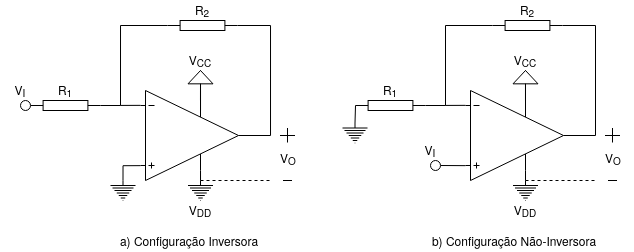
\includegraphics[width=1\columnwidth]{images/fundamentos/AmpOps.png}
    \par\end{centering}

    \label{fig:ampops}
\end{figure}

A figura \ref{fig:ampops} ilustra as configurações mais comuns no uso
de amplificadores operacionais, com uma entrada mantida em um potencial
conhecido. O ganho para a configuração inversora está definido na 
equação \ref{eq:ampop1}, já para a configuração não-inversora, o ganho é 
representado na equação \ref{eq:ampop2}. Para amplificadores de 
instrumentação, o ganho pode ser definido de diversas maneiras, a 
depender do CI empregado.

\begin{equation}
    \label{eq:ampop1}
    V_O = -V_I\left(\frac{R_2}{R_1}\right)
\end{equation}

\begin{equation}
    \label{eq:ampop2}
    V_O = V_I\left(1+\frac{R_2}{R_1}\right)
\end{equation}

As alimentações $V_{CC}$ e $V_{DD}$, observadas na figura \ref{fig:ampops},
são necessárias para o correto funcionamento dos amplificadores em CIs, 
devendo ser respeitados os limites impostos por fabricantes. 
Geralmente a alimentação é simétrica, sendo necessário duas 
fontes de alimentação para que se obtenha o valor correto de saída 
desejado. Todavia, alguns CIs empregam um funcionamento do tipo 
\textit{single-supply}, onde algum dos terminais de alimentação pode 
ser mantido como potencial nulo, ou 0V.
A saída de um circuito do tipo amplificador operacional é limitada 
a uma escala definida por essas duas alimentações, sendo comum esta
escala ser menor que a escala de entrada por alguns volts. 
Amplificadores do tipo \textit{rail-to-rail} permitem que a saída atinja valores mais 
próximos ao valor de alimentação, caso assim seja desejado \cite{mancini2003op}.

Outra maneira de evitar a propagação de interferências da linha ao 
receptor do sinal está no uso de optoacopladores, dispositivos que 
isolam eletricamente o sinal controlador, da carga. A maioria deste 
tipo de equipamento emprega sinais luminosos na faixa de infravermelho 
à luz visível vermelha para o transporte de informação, sem o desgaste
mecânico intrínsico ao funcionamento de relés \cite{temis1996optocouplers}.

\begin{figure}[h]
    \caption{Circuito usual no emprego de optoacoplador.}    
    
    \begin{centering}
        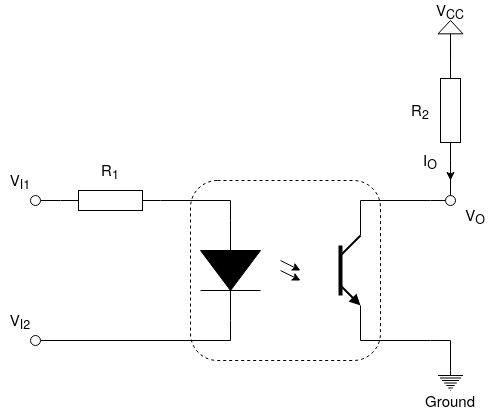
\includegraphics[width=0.6\columnwidth]{images/fundamentos/Optocoupler.png}
    \par\end{centering}

    \label{fig:opto}
\end{figure}

A figura \ref{fig:opto} ilustra o modelo de um optoacoplador, onde o 
sinal de entrada, constituido por $V_{I1}$ e $V_{I2}$ ativa o LED, que
por sua vez causa um sinal luminoso que permita o chaveamento do 
fototransistor \cite{bishop2001understand}. Uma característica importante
sobre o funcionamento de optoacopladores diz respeito à sua taxa de 
transmissão de corrente, isto é, quanto da corrente de entrada o 
dispositivo permite que seja transportado na saída. Denominado como 
CTR, do inglês \textit{Current Transfer Ratio}, esta taxa afeta
diretamente o valor das resistências $R_1$ do circuito, 
pois esta resistência devem ser projetadas de modo que a corrente de 
saída, $I_O$, atinja o valor esperado, e que a corrente de entrada 
esteja sempre no valor de segurança definido pelo fabricante. Caso a 
variável de interesse seja tensão, $V_0$, $R_2$ deve ser inserida no 
circuito com um valor de resistência que resulte em uma diferença de
potencial entre seus terminais de acordo com o desejado.

A corrente de entrada do circuito, ou corrente direta de alimentação 
do diodo, é definida de acordo com a equação \ref{eq:opto1}, em função
da queda de tensão no diodo, $V_f$, sendo possível também expressar a 
resistência $R_1$ em função de uma corrente pré-definida \cite{sedra1998microelectronic}.

\begin{equation}
    \label{eq:opto1}
    I_f = \frac{\left(V_{I1}-V_{I2}\right) - V_f}{R_1}
\end{equation}

Tendo conhecimento da corrente de entrada e do gráfico de CTR para 
determinado positivo, define-se a máxima corrente de saída como
$I_f \cdot CTR$. 

\section{Controle de velocidade}
Uma típica malha de controle pode ser representada em duas formas, denominadas malha aberta ou malha fechada, assim como representado na figura \ref{fig:excontrole},
onde a entrada, ou referência, com interferência ou não da saída, ou variável controlada, alimenta o circuito de controle e este regula o sinal enviado ao processo
para obter assim um valor de acordo com a referência indicada \cite{nise2011control}. 

\begin{figure}[h]
\caption{Formas de representação para controle em malha aberta e malha fechada}    
\begin{centering}
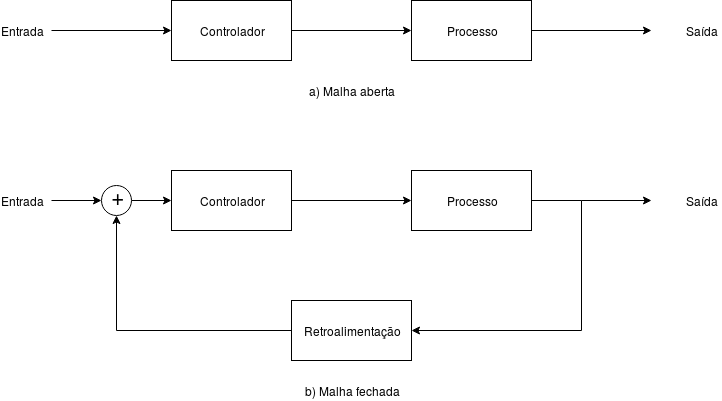
\includegraphics[width=0.8\columnwidth]{images/fundamentos/excontrole.png}
\par\end{centering}

\label{fig:excontrole}
\end{figure}

Em um sistema robótico é comum utilizar alguma malha de controle, como as da figura \ref{fig:excontrole}, para se controlar a posição e/ou velocidade
das juntas do robô, resultando em alguma configuração desejada para este no espaço. 

Para realizar o controle de um manipulador robótico, garantindo
o correto processamento dos dados dos diversos sensores utilizados e o 
acionamento correto dos atuadores, deve ser utilizado um circuito próprio para este fim, como através de um microcontrolador, que 
agrupa em uma mesma placa um processador, memória e portas de entrada e saída de dados, sendo amplamente utilizados em sistemas de medição \cite{bentley2005principles}.
No emprego de um microcontrolador uma importante característica a ser analisada é o seu processador, onde a arquitetura deste afetará
diretamente a implementação do controlador que irá determinar a movimentação do manipulador. Dentre as diversas famílias de processadores, as que mais se 
destacam na área da robótica são ARM, AVR e PIC, além do microcontrolador MSP430. Outra característica a ser analisada na utilização de microcontroladores é 
a quantidade e tipos de periféricos implementados, buscando-se uma unidade que apresente maior aderência com o robô em questão. A frequência de atuação dos
microcontroladores é também de extrema importância na escolha destes, influenciando o tipo de controlador que pode ser implementado, no caso de controladores
digitais.

\subsection{Motores DC}
Para o controle de um motor DC, é necessário inicialmente um modelo
para a representação deste tipo de sistema, sendo um possível modelo 
apresentado na figura \ref{fig:motordc} \cite{krishnan2001electric} \cite{maheriya2016review}.

\begin{figure}[h]
    \caption{Modelo eletromecânico para armadura de motores DC.}    

    \begin{centering}
        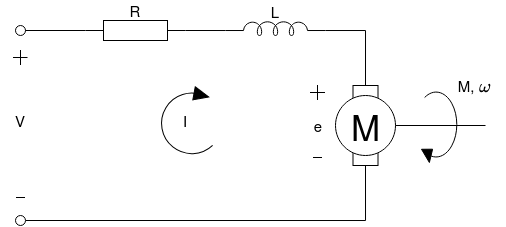
\includegraphics[width=0.6\columnwidth]{images/fundamentos/MotorDC.png} 
    \par\end{centering}

    \label{fig:motordc}
\end{figure}

A figura \ref{fig:motordc} fornece um modelo para o sistema eletromecânico
da armadura de um motor DC, onde uma tensão de entrada, $V$, resulta 
em um torque e velocidade de saída, denominados respectivamente por 
$T$ e $\omega$. A equação elétrica que dita o funcionamento do motor
é expressa em \ref{eq:motordc-eletrico} \cite{krishnan2001electric}.

\begin{equation}
    \label{eq:motordc-eletrico}
    V = e + RI + L \frac{dI}{dt}
\end{equation}

Sabendo que o torque de saída se relaciona com a corrente de entrada
por meio da equação \ref{eq:motordc-torque}, e simplificando a carga
do sistema como um momento de inércia $\mathcal{I}$ e um atrito viscoso, $B$,
obtém-se a equação \ref{eq:motordc-tw} \cite{krishnan2001electric}.

\begin{equation}
    \label{eq:motordc-torque}
    T = K_b I
\end{equation}

\begin{equation}
    \label{eq:motordc-tw}
    T = \mathcal{I}s\omega + B\omega
\end{equation}

Reagrupando as equações de \ref{eq:motordc-eletrico} a \ref{eq:motordc-tw},
é possível observar uma relação entre a velocidade de saída e a tensão
de entrada, ilustrada através da equação \ref{eq:motordc-tf}, no domínio 
de Laplace.

\begin{equation}
    \label{eq:motordc-tf}
    \frac{\omega(s)}{V(s)} = \frac{K_b}{s^2(\mathcal{I}L)+s(BL+\mathcal{I}R)+(BR+K_b^2)}
\end{equation}

A equação em \ref{eq:motordc-tf} fornece um modelo de segunda ordem para
o controle de velocidades de motores DC, entretanto, caso a indutância
do circuito de armadura, $L$, seja desprezível, é possível aproximar 
o modelo proposto como um sistema de primeira ordem.

A fim de controlar a tensão de entrada nestes motores, e consequentemente 
a velocidade de saída, pode-se utilizar um circuito que converta uma tensão
contínua em uma tensão alternada, como através de um circuito do tipo 
\textit{chopper} \cite{krishnan2001electric}.
Circuitos conversores na configuração ponte completa, também conhecidos por 
ponte H completa, ou \textit{Full-H Bridge}, são largamente utilizados na 
geração de níveis de tensão \cite{rashid2017power}, e juntamente com a técnica de controle de 
modulação de largura de pulso - PWM, fornecem um bom meio para controle de 
circuitos análogicos \cite{barr2001pulse}, neste caso, a velocidade, e direção, de um motor DC.

\subsection{Motores de passo}
Motores de passo são, por sua vez, considerados como uma categoria de
motor síncrono, onde a frequência da alimentação que comanda a sua 
velocidade de rotação. Estes motores são utilizados em diversos sistemas
de controle, por oferecem um controle preciso, mesmo em malha 
aberta \cite{chapman2005electric}.  

Embora considerados como máquinas síncronas, os motores de passo são
ativados por uma sequência de chaveamento de suas bobinas que alinham,
a cada passo, o rotor com o campo magnetico gerado no estator. Uma 
relação entre a velocidade de rotação elétrica e a velocidade de rotação do
eixo do motor é proposta em \cite{chapman2005electric} e pode ser vista
na equação \ref{eq:stepper1}, onde $P$ denomina a quantidade de pólos
no motor. 

\begin{equation}
    \label{eq:stepper1}
    \omega_m = \frac{2}{P}\omega_e
\end{equation}

Em \cite{atmel2006stepper}, define-se uma relação mais direta entre 
a velocidade de rotação e o tempo decorrido entre os pulsos enviados por um 
microcontrolador para comando do motor, visível na equação \ref{eq:stepper2}. 
Esta fonte também indica as diferenças básicas entre motores de passo
bipolares e unipolares, bem como no modo de ativação dos motores, com
a possibilidade de uso de configurações de passo completo e meio-passo.

\begin{equation}
    \label{eq:stepper2}
    \omega_m = \frac{\alpha_s}{\delta t} = \frac{\alpha_s}{kt_0}
\end{equation}

Na equação \ref{eq:stepper2}, a constante $\alpha_s$ define o ângulo de passo
básico para determinado motor, ou seja, a variação de rotação na saída 
resultante de um passo na entrada. O termo $\delta t$ informa o período,
em segundos, entre dois pulsos consecutivos para avanço do motor, 
este período pode ser definido como algum múltiplo de um período básico
do microcontrolador, $t_0$, onde somente após decorridos
$k$ períodos internos no controlador, este provocará um pulso para ativação
do motor controlado.

Deste modo, nota-se que o controle de velocidade pode ser realizado
apenas alterando o valor de $k$, através de um contador variável no 
sistema do microcontrolador. Para que motores de passo atinjam determinada
velocidade de uma maneira suave, é necessário que seja realizado um 
controle da aceleração e desaceleração do mesmo, 
variando o valor de $k$ de modo incremental, para que se obtenha uma
rampa de velocidade na saída, com uma aceleração finita \cite{atmel2006stepper}.
Um exemplo de perfil de aceleração pode ser visto na figura \ref{fig:stepperspeed}.

\begin{figure}[h]
    \caption{Exemplo de controle de velocidade para motor de passo.}    

    \begin{centering}
        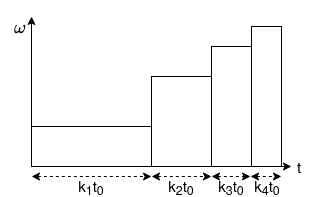
\includegraphics[width=0.5\columnwidth]{images/fundamentos/StepperSpeed.png} 
    \par\end{centering}

    \label{fig:stepperspeed}
\end{figure}

%\subsection{Controle adaptativo}

%\subsection{Controle complacente}

\section{Cinemática de manipuladores}
Um manipulador pode ser analisado como um conjunto de elos conectados
entre si por juntas, e para descrever a relação entre estes elos, 
são definidos sistemas de coordenadas para diferentes partes do 
manipulador, a fim de lidar com a geometrica complexa deste \cite{craig2009introduction}.

Para a correta atribuição de sistemas de coordenadas ao robô, é 
preciso seguir alguma convenção, como aquela definida em \cite{craig2009introduction}.
A convenção apresentada, e que será utilizada ao longo deste trabalho,
define que um sistema de coordenadas será atribuído a cada elo do sistema,
e estes serão numerados de acordo com o elo, onde a base imóvel do robô
é definida como o elo de índice 0. O eixo unitário $\hat{Z}_i$ deve ter a mesma
direção do eixo de rotação do respectivo elo $i$, a origem do sistema 
será posicionada no ponto de intersecção entre o eixo de rotação do elo
um eixo perpendicular a este eixo e o eixo de rotação do próximo elo e o 
eixo $\hat{X}_i$ fica ao longo deste mesmo eixo perpendicular. Por fim, 
o eixo $\hat{Y}_i$ é estabelecido através da regra da mão direita.

Para relacionar matemáticamente os diversos sistemas atribuídos ao 
manipulador, são extraídos parâmetros capazes de relacionar a rotação
e translação entre sistemas de coordenadas consecutivos. Um 
conjunto de parâmetros, utilizado em conjunto com a convenção proposta,
são os parâmetros de Denavit-Hartenberg, ou simplesmente parâmetros de 
DH, em sua forma modificada, estes parâmetros são resumidos do seguinte
modo:

\begin{itemize}
    \begin{centering}
    \item[] $a_i$ = distância entre $\hat{Z}_i$ e $\hat{Z}_{i+1}$, ao longo de $\hat{X}_i$;
    \item[] $\alpha_i$ = ângulo entre $\hat{Z}_i$ e $\hat{Z}_{i+1}$, em relação a $\hat{X}_i$;
    \item[] $d_i$ = distância entre $\hat{X}_{i-1}$ e $\hat{X}_i$, ao longo de $\hat{Z}_i$;
    \item[] $\theta_i$ = ângulo entre $\hat{X}_{i-1}$ e $\hat{X}_i$, em relação a $\hat{Z}_i$.
    \par\end{centering}
\end{itemize}

Percebe-se que para representar a posição e orientação do sistema de 
índice $i$ em relação ao sistema $i-1$, são necessários os parâmetros 
$\alpha_{i-1}$, $a_{i-1}$, $d_i$ e $\theta_i$. 
A equação \ref{eq:transform} ilustra a transformação necessária
para representar um vetor em coordenadas homogêneas definido no 
sistema de coordenadas $i$, em relação ao sistema $i-1$.

\begin{equation}
    \label{eq:transform}
    ^{i-1}_iT = 
    \begin{bmatrix}
        cos\theta_i                 & -sen\theta_i                  & 0                 & a_{i-1}               \\
        sen\theta_icos\alpha_{i-1}  & cos\theta_icos\alpha_{i-1}    & -sen\alpha_{i-1}  & -sen\alpha_{i-1}d_i   \\
        sen\theta_isen\alpha_{i-1}  & cos\theta_isen\alpha_{i-1}    & cos\alpha_{i-1}   & cos\alpha_{i-1}d_i    \\
           0                        &    0                          &    0              &  1                    \\    
    \end{bmatrix}
\end{equation}

A transformação exposta em \ref{eq:transform} é composta pela junção
de uma matriz de rotação, $^{i-1}_iRot$, um vetor de translação, $^{i-1}Pos_i$,
e uma linha extra composta por três zeros e um único um,
a fim de transformar a matriz em uma matriz quadrátrica, facilitando
a inversão da transformação, como indicado na equação \ref{eq:transform2}. 

\begin{equation}
    \label{eq:transform2}
    ^{i-1}_iT = 
    \begin{bmatrix}
        ^{i-1}_iRot & ^{i-1}Pos_i   \\
        0 \;\; 0 \;\; 0       & 1   \\
    \end{bmatrix}
\end{equation}

A notação adotada para os índices 
sobrescritos e subescritos se manterá a mesma ao longo de todo este
documento, onde o índice sobrescrito precedente denota o sistema de 
coordenadas de referência de referência desejado, e o índice subescrito 
precedente informa o sistema de coordenadas original.

\subsection{Propagação de velocidades}
É possível definir a velocidade angular e linear de determinado 
sistema de referência no manipulador em função da movimentação desta
junta e da movimentação de juntas passadas. Através dos cálculos 
desenvolvidos em \cite{craig2009introduction}, são obtidas 
equações para a propagação de velocidades entre juntas, referenciadas
nas equações \ref{eq:speed1} e \ref{eq:speed2}.

\begin{equation}
    \label{eq:speed1}
    ^{i+1}\omega_{i+1} = \; ^{i+1}_iRot\,^i\omega_i + \dot{\theta}_{i+1}\,^{i+1}\hat{Z}_{i+1}
\end{equation}

\begin{equation}
    \label{eq:speed2}
    ^{i+1}v_{i+1} = \; ^{i+1}_iRot\left(^iv_i+^i\omega_i\times ^iPos_{i+1}\right)
\end{equation}

As equações \ref{eq:speed1} e \ref{eq:speed2} dizem respeito à velocidades
geradas por juntas de rotação. A velocidade angular pode ser vista 
como uma soma entre a velocidade angular da junta precedente, 
termo $^{i+1}_iRot\,^i\omega_i$, e a rotação gerada pelo próprio eixo,
$\dot{\theta}_{i+1}\,^{i+1}\hat{Z}_{i+1}$. 
A velocidade linear, por sua vez, é a soma da velocidade linear da 
junta precedente com a resultante linear da multiplicação vetorial
entre a velocidade angular da junta precedente com o deslocamento, 
ambos representados no novo sistema de coordenadas, $i+1$.

\subsection{Jacobiana}
\label{sec:jacobiana}

Aplicando-se as equações \ref{eq:speed1} e \ref{eq:speed2} para as juntas
de um manipulador, é possível obter as velocidades de cada elo em função
dos termos $\dot{\theta}_i$, agrupando-se estas relações em uma forma matricial,
gera-se uma representação entre as velocidades das juntas e as velocidades
lineares e angulares de diversos elos. À matriz resultante deste 
agrupamento, que relaciona variações temporais na entrada com 
a saída, relação visível na equação \ref{eq:mjacobiana}, atribui-se o 
nome de Jacobiana \cite{craig2009introduction}.

\begin{equation}
    \label{eq:mjacobiana}
    \dot{Y} = J(X)\dot{X}
\end{equation}

Em certos casos, a matriz Jacobiana pode ser organizada com a sua 
inversão em mente, para que se obtenha a velocidade que deve ser 
imposta nas juntas de um robô para gerar determinadas velocidades
lineares e angulares desejadas.